\documentclass[10pt,a4paper]{article}
	\usepackage[utf8]{inputenc}
	\usepackage{amsmath}
	\usepackage{amsfonts}
	\usepackage{amssymb}
	\usepackage{graphicx}
	\usepackage{diagbox}
	\usepackage{tikz-cd}
	\usepackage{csquotes}
	\usepackage{marginnote}
	\author{Jiren Zhu}
	\title{Understanding Libratus, the algorithm that beats world-class poker players}
	\newcommand{\calA}{\mathcal{A}}
	\newcommand{\calB}{\mathcal{B}}
	\newcommand{\calD}{\mathcal{D}}
	\newcommand{\calF}{\mathcal{F}}
	\newcommand{\calP}{\mathcal{P}}
	\newcommand{\bbI}{\mathbb{I}}
	\newcommand{\bbP}{\mathbb{P}}
	\newcommand{\bbE}{\mathbb{E}}
	\newcommand{\bbR}{\mathbb{R}}
	\newcommand{\bE}{\bold{E}}
	\newcommand{\bP}{\bold{P}}
	\newcommand{\bQ}{\bold{Q}}
	\DeclareMathOperator*{\argmin}{argmin}
	\DeclareMathOperator*{\argmax}{argmax}
	\usepackage{tikz-qtree}
	\tikzset{
		% Two node styles for game trees: solid and hollow
		solid node/.style={circle,draw,inner sep=2,fill=black},
		hollow node/.style={circle,draw,inner sep=2},
		empty node/.style={rectangle,draw,fill=white,color=white},
		random node/.style={rectangle,draw,inner sep=2}
	}
	
	% macro for entering payoffs
	\newcommand\payoff[1]{
		$\begin{pmatrix} #1 \end{pmatrix}$
	}
\begin{document}
\maketitle
% \setcounter{secnumdepth}{0}

% \section{Introduction}
In January 2017, four world-class poker players engaged in a three-week battle of heads-up no-limit Texas hold'em. However, they were not competing against each other. Instead, they were fighting against a common foe: an AI called ``Libratus'', developed by Noam Brown and Tuomas Sandholm from Carnegie Mellon University. As the game progressed, the computer held a solid advantage, beating the humans with $99.98\%$ statistical significance \cite{brown2017superhuman}. \marginnote{What metric for significance?} This is one of the first AI agents to beat professional players in heads-up no-limit Texas hold 'em \footnote{Concurrently, DeepStack \cite{moravvcik2017deepstack} has been shown to beat professionals as well.}. Unlike other recent human-level AI agents, Libratus did not use Reinforcement Learning or Deep Learning, two approaches that are extremely popular these days. Instead, Libratus used a classical game-theoretic approach. It is natural to ask: what did Libratus do to play the game? What challenges did it face? And how did it overcome them? To get an answer to these questions, we first need to look at the game of poker itself. 
\marginnote{Good opportunity here to mention that poker is more like the ``real world'' than other games}

\section{Game, Games}
Libratus is definitely not the only game-playing AI to make news headlines in recent years. In 2015, for instance, DeepMind's DQN beat a number of Atari ``games'', achieving superhuman performance~\cite{mnih2015human}. However, these two games are rather different. [The Atari games DQN beat are all single-player games, while poker is a multiplayer game. Thus the two AIs have very different designs:] DQN is a decision process best understood under the reinforcement learning framework, where a \textit{single} agent makes decisions. Libratus, on the other hand, is developed under game theory, where \textit{more than one} decision makers interact. 

The presence of multiple decision makers makes the story very different. In a single-agent decision process, there is a unique best policy. But in a multi-party game, the notion of optimality is different. Your opponent's strategy matters. Using your favorite strategy against Alice may yield a different reward than using it against Bob. In fact, one of the most important concepts of game theory, the Nash equilibrium, is precisely a way to define an ``optimal'' strategy in this situation. We will introduce it first, as it is crucial to understanding the game-theoretic design of Libratus.

\subsection{Normal form games and Nash equilibria}

Before we define the Nash equilibrium, we need a more formal definition of games under game theory. A very simple yet very important type of game is the \textit{normal form game}. In a normal form game, each player has a collection of available actions: $A_1$ for Player 1, and $A_2$ for Player 2. (For our purpose, we will limit our discussion to two-player games only.) The two players simultaneously choose actions $a_1 \in A_1$, $a_2 \in A_2$ and receive rewards $u_1(a_1, a_2)$, $u_2(a_1, a_2)$, where $u_1$ and $u_2$ are functions over the actions of both players.

As an example, let's look at how rock-paper-scissors would look like under this formulation. There are three actions available to both players: let's use $R$ for rock, $P$ for paper and $S$ for scissors. We will also assume that for both players, winning a game would yield one dollar in return and losing will yield -1. A draw would mean 0 return for both players. The game would then look like Figure~\ref{figure:RPS}. To see the outcome of a game, we would go to the row corresponding to action of Player 1 and column corresponding to Player 2. Say that Player 1 plays paper and Player 2 plays rock. We would find the $P-R$ cell and get $1/-1$. These numbers correspond to the rewards received by Player 1 and Player 2, respectively. Player 1 wins a dollar, Player 2 loses one. Paper beats rock.

A \textit{strategy} describes how each player chooses his actions. If a player chooses strategies deterministically, the strategy is called a \textit{pure strategy}, and a strategy that involves some randomness is called a \textit{mixed strategy}. We usually describe a mixed strategy as a probability distribution over all actions, using $\sigma_1(a)$ to describe the probability that Player 1 plays action $a$. Thus the expected payoff for this player is
$$
	u_1(\sigma_1, \sigma_2) := \sum_{a_1 \in A_1, a_2 \in A_2} u_1(a_1, a_2)\sigma_1(a_2)\sigma_2(a_2)
$$

\begin{figure}[ht]
	\centering
	\begin{tabular}{|c|c|c|c|}
		\hline
		  & P    & S    & R    \\ \hline
		P & 0/0  & -1/1 & 1/-1 \\ \hline
		S & 1/-1 & 0/0  & -1/1 \\ \hline
		R & -1/1 & 1/-1 & 0/0  \\ \hline
	\end{tabular}
	\caption{Normal form game formulation of rock-paper-scissors}
	\label{figure:RPS}
\end{figure}

\paragraph{Nash and Nash equilibrium}
It is time that we introduce Nash, perhaps the most important figure in Game Theory. John Nash is a genius mathematician who laid the foundation of this thriving subject. \marginnote{Not sure if the bit about John Nash needs to be here. Maybe in the caption of a photo of Nash?} Perhaps the most fundamental concept in game theory is that of a Nash equilibrium, which Nash described. A \textbf{Nash equilibrium} is a scenario where none of the participants of a game can improve his/her outcome by changing only his/her own strategy. Formally speaking, a Nash equilibrium consists of strategies $\sigma_1$ and $\sigma_2$ such that if Player 1 chooses another strategy $\sigma_1'$, we have
$$
	u_1(\sigma_1, \sigma_2) \geq u_1(\sigma_1', \sigma_2)
$$
and vice versa for Player 2. This captures the fact that a rational player would do whatever is in his/her control to maximize the outcome from a game.
\marginnote{Maybe say something about why a Nash equilibrium is ``optimal''?}

Nash's important contribution is his proof of the \textit{Nash existence theorem}, which showed that there always exists a mixed strategy Nash Equilibrium for games with finite numbers of actions. For this reason, one usually considers mixed strategies when talking about games (as otherwise a Nash equilibrium may not even exist).

\subsection{Zero-sum games}
An shared feature among poker, rock-paper-scissors, and many other competitive games is that whatever one player gets is the negative of what the other player gets. Such a game is called a \textit{zero-sum game}. Formally speaking, for all $a_1 \in A_1$ and $a_2 \in A_2$, we have this equation:
$$
	u_1(a_1, a_2) + u_2(a_1, a_2) = 0
$$
An important property of zero-sum games is that any Nash equilibrium can be computed efficiently. The \textbf{maxmin} value for Player 1 is the maximum payoff that Player 1 can guarantee regardless of what action Player 2 chooses:
$$
	\max\min_1 = \max_{a_1}(\min_{a_{2}} u_1(a_1, a_{2}))
$$
The corresponding \textbf{minmax} value of Player 1 is the minimum payoff that Player 2 can force Player 1 into taking, if Player 2 chooses his/her action first:
$$
	\min\max_1 = \min_{a_2}(\max_{a_{1}} u_1(a_1, a_{2}))
$$

The \textbf{Minmax theorem} states that minmax and maxmin are equal for a zero-sum game (with mixed strategies) \marginnote{Why do we discuss minmax at all?} and that Nash equilibria consist of both players playing maxmin strategies. An important corollary is that \textit{the Nash equilibria of zero-sum games can be computed efficiently} since the maxmin strategy can be solved by a linear program maximizing $v$ over $v \in \bbR$, $\sigma_1$ a probability distribution over $A_1$, satisfying
$$
	\sum_{a_1}\sigma_1(a_1)u_1(a_1, a_2) \geq v\ \forall a_2 \in A_2
$$

\newpage
\section{More complicated games}
\subsection{Extensive form games}
While many games fall in the category of normal form games, many more do not. In a normal form game, two players each take one action simultaneously. But games like poker, chess, and tic-tac-toe involve players taking turns and making a series of moves. A more general formalism is necessary \footnote{Technically, an extensive form perfect information game can still be casted back to a normal form game where the actions are different strategies. But this normal form game would be very large and redundant.} for studying these games. Thus, games like poker are usually studied as \textit{extensive form games}, where multiple actions may take place one after another. 

See Figure~\ref{figure:ExtensiveFormGame} for an example. Player 1 first takes action between $L$ and $R$. $R$ ends the game with payoff $(5,2)$. $L$ continues the game, offering Player 2 choice between $l, r$ and corresponding rewards. All the possible games states are specified by the game tree, and it is relatively easy to read off what is going on.

\begin{figure}[ht]
	% https://gist.github.com/cdcrabtree/8134418
	\centering
	\begin{tikzpicture}
		[every level 0 node/.style={draw,hollow node},
			every level 1 node/.style={draw,solid node},
			every level 2 node/.style={draw,empty node},
			every level 3 node/.style={draw, empty node},
			grow=down,
			level distance=.85in,
			sibling distance=.65in,
			edge from parent path={(\tikzparentnode) -- (\tikzchildnode)}
		]
		\tikzstyle{edge from parent}=[draw,black,thick]
		\Tree [
		.\node [ label=left:{{1}}]{};
		\edge node [auto=right] {L};
		[ .\node[label=left:2]{};
		\edge node [auto=right] {l}; [.\node [label=right:{\payoff{2, 6}}] {};]
		\edge node [auto=left] {r}; [.\node [label=right:{\payoff{3, 6}}] {};]
		]
		\edge node [auto=left] {R};
		[.\node [draw,fill=white,color=white,label=right:{\payoff{5, 2}}] {};]
		]
		]
	\end{tikzpicture}
	\caption{A game tree of extensive form game}
	\label{figure:ExtensiveFormGame}
\end{figure}

Another very good example of an extensive form zero-sum game is Go. Figure $3$ shows a game tree where we parameterize the location of the piece by its coordinate.

\begin{figure}[ht]
	% https://gist.github.com/cdcrabtree/8134418
	\centering
	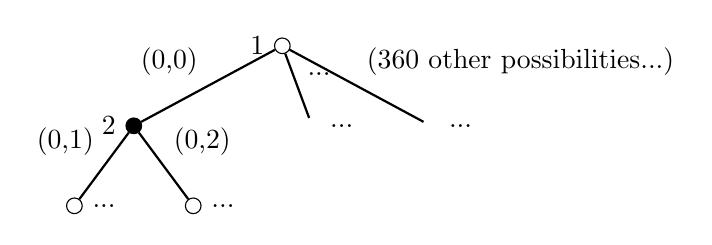
\begin{tikzpicture}
		[every level 0 node/.style={draw,hollow node},
			every level 1 node/.style={draw,solid node},
			every level 2 node/.style={draw,hollow node},
			every level 3 node/.style={draw, solid node},
			grow=down,
			level distance=.4in,
			sibling distance=.3in,
			edge from parent path={(\tikzparentnode) -- (\tikzchildnode)}
		]
		\tikzstyle{edge from parent}=[draw,black,thick]
		\Tree [
		.\node [ label=left:{{1}}]{};
		\edge node [auto=right] {(0,0)};
		[ .\node[label=left:2]{};
		\edge node [auto=right] {(0,1)}; [.\node [label=right:{...}] {};]
		\edge node [auto=left] {(0,2)}; [.\node [label=right:{...}] {};]
		]
		\edge node [auto=left] {...};
		[.\node [draw,fill=white,color=white,label=right:{...}] {};]
		\edge node [auto=left] {(360 other possibilities...)};
		[.\node [draw,fill=white,color=white,label=right:{...}] {};]
		]
		]
	\end{tikzpicture}
	\caption{A partial game tree of Go}
	\label{figure:Go}
\end{figure}

One immediately notices that it is hard to even specify a small portion of the game tree, as the number of possibilities grows exponentially fast. Even worse, while zero-sum games can be solved efficiently, a na\:{i}ve approach is polynomial in the number of pure strategies---and this number grows exponentially with respect to the size of game tree. Thus, finding an efficient representation of an extensive form game is a big challenge for game-playing agents. For example, AlphaGo~\cite{silver2017mastering} used neural networks to represent the outcome of a subtree of Go. Similarly, a lot of innovations in Libratus are novel ways to abstract the game to a reasonable size while preserving relevant information.

\subsection{Imperfect information games}

[To those unfamiliar with game theory, it might come as a surprise that computers would beat humans at both chess and Go before heads-up no-limit Texas hold 'em.] While Go and poker are both extensive form games, the key difference is that Go is a \text{perfect information game}, while poker is an \text{imperfect information game}. In a game of poker, cards are dealt randomly, and players can only observe some of them. 

To visualize the game tree of an imperfect information game, we use \textit{chance nodes}. For instance, Figure~\ref{figure:imperfectinformation} is a simplified game tree for poker. Here, randomness is depicted by the chance nodes $R_1$ and $R_2$.

\begin{figure}[ht]
	% https://gist.github.com/cdcrabtree/8134418
	\centering
	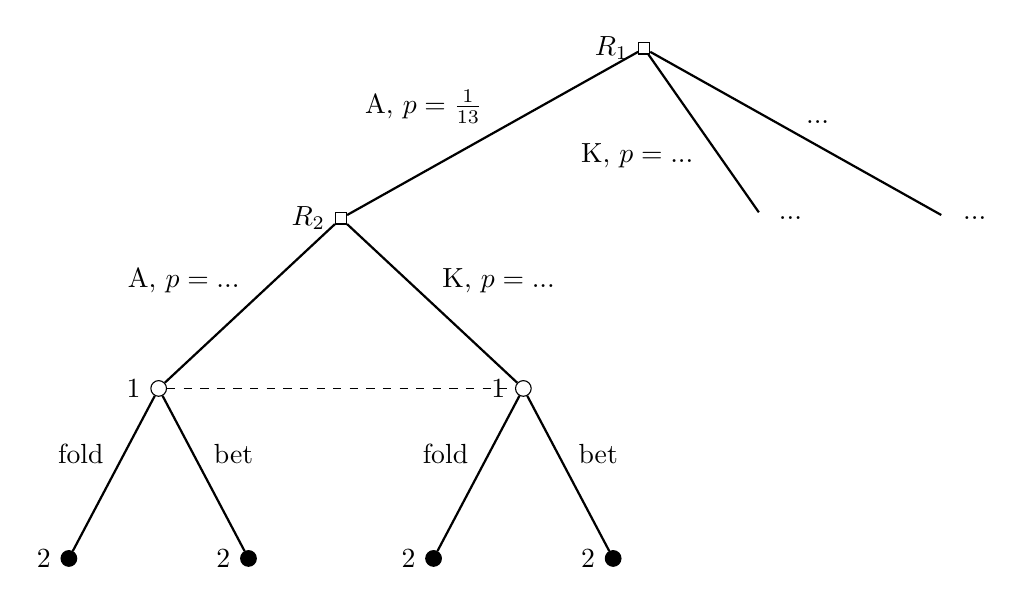
\begin{tikzpicture}
		[
			every level 0 node/.style={draw,random node},
			every level 1 node/.style={draw,random node},
			every level 2 node/.style={draw,hollow node},
			every level 3 node/.style={draw,solid node},
			every level 4 node/.style={draw, empty node},
			grow=down,
			level distance=.85in,
			sibling distance=.65in,
			edge from parent path={(\tikzparentnode) -- (\tikzchildnode)}
		]
		\tikzstyle{edge from parent}=[draw,black,thick]
		\Tree [
		.\node [ label=left:$R_1$]{};
		\edge node [auto=right] {A, $p = \frac{1}{13}$};
		[ .\node[label=left:$R_2$]{};
		\edge node [auto=right] {A, $p = ...$};
		[ .\node [ label=left:1 ] (P1-A-A) {};
		\edge node [auto=right] {fold};
		[.\node [ label=left:2 ] {};]
		\edge node [auto=left] {bet};
		[.\node [ label=left:2 ] {};]
		]
		\edge node [auto=left]  {K, $p = ...$};
		[ .\node [label=left:1] (P1-A-K) {};
		\edge node [auto=right] {fold};
		[.\node [ label=left:2 ] {};]
		\edge node [auto=left] {bet};
		[.\node [ label=left:2 ] {};]
		]
		]
		\edge node [auto=right] {K, $p = ...$};
		[.\node [draw,fill=white,color=white,label=right:{...}] {};]
		\edge node [auto=left] {...};
		[.\node [draw,fill=white,color=white,label=right:{...}] {};]
		]
		]
		\draw [dashed] (P1-A-A) -- (P1-A-K) ;
	\end{tikzpicture}
	\caption{A game tree of imperfect information game, Player 1 cannot distinguish which $\circ$ he/she is in.}
	\label{figure:imperfectinformation}
\end{figure}

In this simplified game tree, a random card is first dealt to Player 1 with some probability specified at chance node $R_1$. Then, another random card is dealt to Player 2 at chance node $R_2$. Finally, it is Player 1's turn to bet. 

\textit{Note that Player 1 does not have perfect information.} He does not know what card is dealt to Player 2. In the game tree, this is denoted by the dashed line between the two states, or the \textit{information set}. An information set is a collection of game states that a player cannot distinguish between when making decisions. In an imperfect information game, each player must have only one strategy in each information set. [\textit{The meaning of this sentence is unclear. Did we define extended-form strategies?}] When Player 1 finds himself in a certain information set, the true state of the world can only be guessed as a distribution over all possibilities specified by that information set. To decide his next action, he needs to evaluate the payoffs of each action over all possible underlying states.

Imperfect information makes a crucial difference in decision making. A Go-playing agent asks itself the question: ``based on the \textbf{current state} of the game, what should I do?'' But a poker agent has to make a decision based on an estimate: ``based on my current observations, what is the \textit{estimated distribution} of all possible ground truth states of the game, and what is the \textit{best action} based on that distribution?'' 

\marginnote{I'm not sure if I get this ``important difference''. It seems to come from the extended form assumption and not necessarily the imperfect information one?} The important difference follows. Because the opponent is making decisions as well, if you change your strategy at observed state $s$, he may change his action, and the model for opponent, namely the distribution $\sigma$, that you used to find the new strategy is no longer valid, and your strategy no longer works. 

We shall follow \cite{bowling2015heads} and use a quote from Von Neumman to explain the difference between perfect and imperfect information:

\begin{displayquote}
	Real life is not like that. Real life consists of bluffing, of little tactics of deception, of asking yourself what is the other man going to think I mean to do. And that is what games are about in my theory.
\end{displayquote}

\newpage
\section{Poker and Libratus}
Now that we have the necessary game theoretic terminology, let's take a look at Poker and why Poker is such a challenge. In Poker, each players are dealt cards that are secret to the other player, so the game is an imperfect information game. The variant of Poker that Libratus solved is called heads up no-limit Texas Hold'em. Heads up means that there are only two players playing against each other, making the game a two-player zero sum game.

As described in \cite{brown2017superhuman}, Libratus has three main modules, game abstraction, subgame solving and self improvement. We shall discuss them in the next three sections.

\subsection{Game abstraction}
No-limit means that there is no fixed bet sizes and no limit on the number of raises. In contrast, in a limited version of the game, bet sizes are fixed and number of raises are fixed. This reduces the number of possibilities of the game state, which makes the game easier to solve. This variant is solved in 2015 by \cite{bowling2015heads}.

As a comparison, the limit version has $1.38 \times 10^{13}$ information sets. According to the report, to solve the limited version, an algorithm, named ``CFR+'', ``was executed on a cluster of 200 computation nodes each with 24 2.1-GHz AMD cores, 32 GB of RAM, and a 1-TB local disk. The algorithm takes 61 min on average to complete one iteration. The computation was then run for 1579 iterations, taking 68.5 days, and using a total of 900 coreyears of computation (43) and 10.9 TB of disk space, ...''. This is already a lot of computation.

In the no limit version, a bet size can be $\$ 501$ or $\$ 502$ and they are different game states. This results in a whopping $10^161$ different decision points from a naive view of the game. Nevertheless, it is not necessary to construct a new betting strategy for a single dollar difference  in the bet. One of the first task that Libratus must accomplish is to abstract the game to bring it down to a more realistic abstraction.

Libratus abstracts the game by grouping similar actions and similar cards, bring the game size down to $10^{12}$ \cite{brown2017superhuman}. This results in a manageable game that can thus be solved by a variation of the CFR method. The abstraction is referred to as the \textbf{blueprint}.

\paragraph{Solving the blueprint: Counterfactual Regret Minimization}
Recall that earlier we mentioned that Nash equilibriums in normal form two player zero sum games can be solved by linear program. The ideal can be directly applied to an extensive form game where a possible strategy of a player describes what he does in all information sets. This approach, however, does not apply to any game of reasonable size as such possible strategies grow exponentially with respect to the number of information sets. Later methods exploits the tree-like structure of extensive form games and represent strategies as the actions at each node.

Counterfactual Regret Minimization (CFR) is an iterative algorithm that solves for Nash equilibriums in extensive form games that has linear run time with respect to the number of information sets. In CFR methods, two agent play against each other and tries to minimize its own counterfactual regret with respect to the other agent's current strategy. Libratus uses a Monte Carlo based variant where they sample the game tree to get an approximate return for the subgame rather than enumerating every leaf node of the game tree. Additionally, they apply pruning so that the algorithm does not sample really bad actions. For more information, see~\cite{zinkevich2008regret, johanson2012efficient}

\subsection{Nested safe subgame solving}
While many Poker bots use an abstraction of the game to reduce the size of the game, they typically stick to the abstraction. Suppose that the blueprint evaluates the scenarios where the opponent bets $\$100$ and $\$200$ beforehand. If the opponent bets $\$134$ in the actual game, the bot would treat it as if the opponent bet $\$100$ through rounding.

Libratus takes an alternative approach. It expands the game tree at the off-blueprint action in real time and solves for that subgame exactly. This method, ``subgame solving'', was proposed earlier but were not shown to improve the performance of an agent. The difficulty originates from the fact that different subtrees in the game state are not independent in an imperfect information game, and you cannot look at a subgame in isolation.

In a perfect information normal form game, if you have reached a subgame, your best strategy in this subgame is independent of what you do in other subgames. When you are holding a pair of $K$ and your opponent calls your blind, there are multiple possible situations, maybe he has $2$ and $7$, or he has a pair of $A$. All of his possible actions form a propability distribution conditioned on this information set being reached. But your opponent's action depends on how this subgame compares to other subgames. And if the opponent changes his strategy according to your new strategy in the subgame, the probability distribution of his possible hands at this information set would be different. This effectively invalidates the previously solved best strategy.

``Unsafe'' subgame solving refers to the naive approach where one assumes that the opponent's strategy is fixed and computes a best strategy for the subgame. A ``safe'' subgame solving method augments the subgame by augmenting the subgame by giving Player 1 some alternatives where he can choose not to enter the subgame being solved and receive expected payoff under the blueprint. This ensures that for any possible situation, Player 1 is no better-off reaching the subgame after the new strategy is computed. This requirement turns out to be too conservative. Libratus uses ``reach'' subgame solving which only requires that Player 1 becomes no better off for those cases where he is likely to reach this subgame.

\subsection{Self improvement}
Finally, during the day when Libratus is playing against human players, it looks for most frequent off-blueprint actions. At night, Libratus refines its blueprint to solve for equilibrium of these actions. Thus Libratus continuously narrows the gap between actions taken by the human players and its blueprint abstraction of the game. This way, as the game goes on, it is harder and harder to exploit the fact that Libratus is only solving an approximate version of the game.

\section{Final words}
While Libratus only beat professionals in a game setting, its importance goes beyond playing Poker. Game theory is widely used in economics. Many real life scenarios can be well characterized as a game. Whether it is companies setting prices, generals positioning armies or employees negotiating wages there are more than one decision makers trying to maximize output. Other applications of game theory include school matching, liver matching, elections, road planning and evolutionary biology. Being able to solve complex imperfect information games at superhuman level means that agents may help humans in all these tasks. It is really exciting to see that the methodologies of Libratus can be applied and actually improve the well being of people around the globe.


\newpage
\bibliography{main}
\bibliographystyle{ieeetr}

\end{document}

\begin{figure}[p]
	\includegraphics{image.png}
\end{figure}

% % % % 
% table
% % % % 
\begin{center}
	\begin{tabular}{|c|cc|}
		\hline
		\diagbox{1}{2} &  & \\
		\hline
		               &  & \\
		               &  & \\
		\hline
	\end{tabular}
\end{center}

$$\lessim$$